\documentclass[conference]{IEEEtran}
\IEEEoverridecommandlockouts
% The preceding line is only needed to identify funding in the first footnote. If that is unneeded, please comment it out.
\usepackage{cite}
\usepackage{amsmath,amssymb,amsfonts}
\usepackage{algorithmic}
\usepackage{graphicx}
\usepackage{hyperref}
\usepackage{epstopdf}
\usepackage{epsfig}
\usepackage{glossaries}
\usepackage{textcomp}
\usepackage{xcolor}
\def\BibTeX{{\rm B\kern-.05em{\sc i\kern-.025em b}\kern-.08em
    T\kern-.1667em\lower.7ex\hbox{E}\kern-.125emX}}

\newacronym{batman}{B.A.T.M.A.N.}{Better Approach To Mobile Adhoc Networking}
\newacronym{rtt}{RTT}{Round Trip Time}
\newacronym{arq}{ARQ}{Automatic Repeat-reQuest}
\newacronym{ne}{NE}{Nash Equilibrium}

\begin{document}

\title{A game-theoretical analysis of BATMAN-adv protocol}

\author{\IEEEauthorblockN{Andrea Pittaro}
\IEEEauthorblockA{\textit{Dipartimento di Ingegneria dell'Informazione} \\
Padova, Italy \\
andrea.pittaro@studenti.unipd.it}
\and
\IEEEauthorblockN{Enrico Lovisotto}
\IEEEauthorblockA{\textit{Dipartimento di Ingegneria dell'Informazione} \\
Padova, Italy \\
enrico.lovisotto@studenti.unipd.it}
}

\maketitle

\begin{abstract}

\end{abstract}

\section{Introduction}

\section{State of the art}

\gls{batman} was born in 2007 as a mesh networks protocol that allowed users to
create network using their devices as nodes that routes traffic and transmit
data to the network.

In 2008 \gls{batman} Advanced specification was released: exploiting channel
knowledge present at ISO/OSI layers 2 and 3, and so breaking the logical
separation of entities in the stack, the module can route the incoming packets
more efficiently.

During these years the standard evolved, thanks to the testing campaign promoted
by the Freifunk\footnote{See project website at \url{https://freifunk.net/en/}}
initiative, whose goal is the creation of a decentralized WiFi network all
across Germany.

Finally, in 2011 \gls{batman} became officially supported by the Linux Kernel,
allowing all PCs to become a node in the network.

- how does the protocol work: principles

\section{Methodology}

\subsection{Network setup}

In order to assess and verify the expected properties of the \gls{batman}
protocol, we decided to run an event-driven simulation.

So, a certain number of entities were scattered uniformly across the simulation
area, as shown in \autoref{fig:nodes}. This strategy allows to change topology
simply switching the generator random seed and will be used for validating all our results.

\begin{figure}[h]
  \centering
  \hspace{-0.7cm}%
  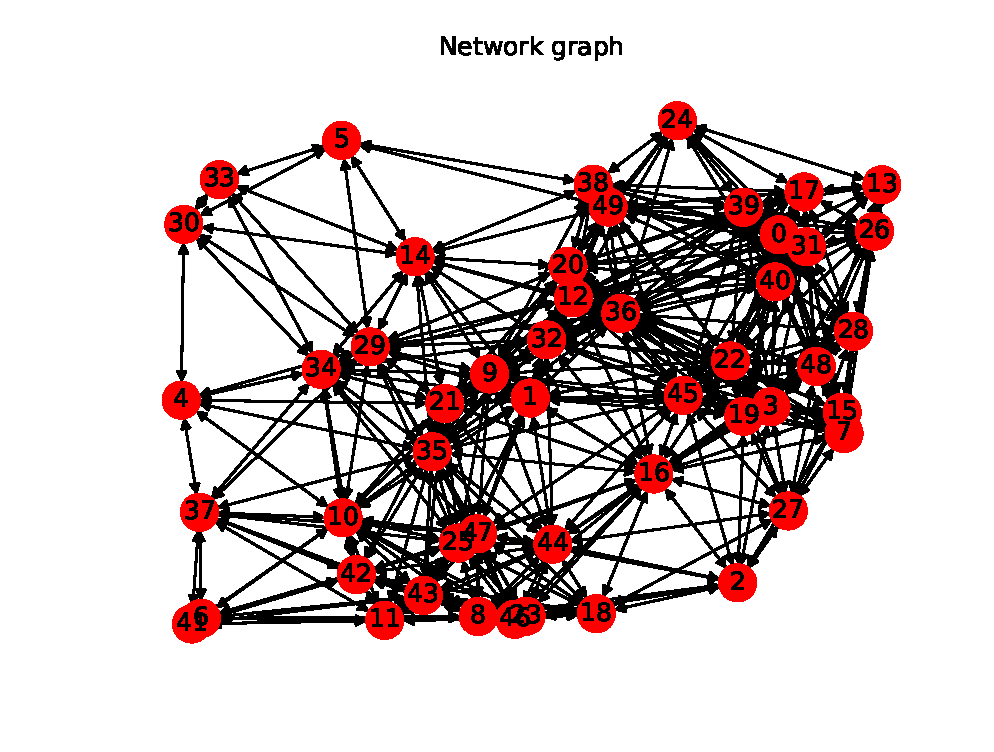
\includegraphics[width=1.1\linewidth]{figures/example_graph}
  \caption{Nodes, labeled by their IP, are connected each other wirelessly.}
  \label{fig:nodes}
\end{figure}

Once placed, each couple of nodes close enough were linked by means of a
wireless fully reliable channel, characterized by a \gls{rtt} and a
retransmission probability $p_r$, both function of the reciprocal distance.

This assumption on the channel characteristics reduces the model complexity
while keeping an high degree of realism, as \gls{arq} strategies are common
practice at all protocol stack levels.

\begin{equation}
  \begin{split}
    p_r & = e^{-\frac{d}{D}} \\
    RTT &= 2 \frac{d}{c_0} + t_{proc}
  \end{split}
\end{equation}

Given previous hypothesis, communication can be described by message exchange in
a directed graph made of \gls{batman}, channels and application layers, as shown
in \autoref{fig:graph}.

\begin{figure}[h]
  \centering
  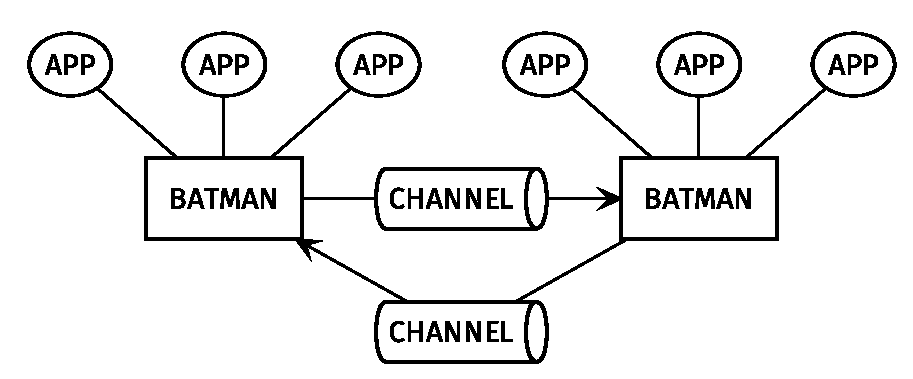
\includegraphics[width=\linewidth]{figures/layers_diagram}
  \caption{Abstract graph spanning all logical components of the network.}
  \label{fig:graph}
\end{figure}

\subsection{Expected results}

In order to be as general as possible, our network connects memoryless sources
of traffic communicating to each other: the \gls{batman} layer has the goal to
serve its users as best as it can. To do so, node have to rely to a certain
extent on their neighbours, since not all destinations are reachable in a single
hop.

From a game theoretical point of view, two different strategies can be chosen by
each layer in order to maximize its objective: either it can collaborate with
its own kind, using part of its bandwidth to forward packets of other sources,
or selfishly transmit only its own packets.

As we will show in the upcoming \autoref{sec:results}, the protocol is designed
in such a way that the altruistic path is more convenient for the nodes to
pursue. The collaboration will turn out to be, in fact, a \gls{ne} for the game
played between all the connected entities.

We will furthermore analyze in which terms the network can sustain itself when a
growing fraction of its users are selfish or network conditions degrade.

% TODO bit of spoilers for results section

\section{Results} \label{sec:results}

Network performances between fair and unfair users varying
- percentage of unfair users
- requested traffic (number and intensity of apps)
- channel quality

\section{Conclusion}

\bibliography{report}
% \bibliographystyle{IEEEtran}

\end{document}

%%% Local Variables:
%%% mode: latex
%%% TeX-master: t
%%% End:
